%!TEX root = kotov.tex
\section{Task 1: Дерево Штайнера}
\begin{task}
    Дан взвешенный неориентированный граф $G = \braket{V, E}$.
    В графе есть подмножество вершин~$T$,
    которые мы назовем терминалами.
    Минимальное дерево Штайнера --- это связный подграф графа $G$ минимального веса, содержащий все терминалы.
    Требуется найти такое дерево.
	\begin{enumerate}
        \item Пусть $|T| = 3$, решить за $\O(E \log V)$.
        \item Пусть $|T| = 4$, решить за $\O(V^3)$.
	\end{enumerate}
\end{task}

\begin{solution}
    \begin{enumerate}
        \item У нас из чатика добавилось условие, что веса неотрицательные, это важно нам, чтобы можно было запускать алгоритм Дейкстры.
        Запустим для каждой терминальной вершины алгоритм Дейкстры, на выходе мы будем знать расстояния от каждой терминальной вершины до любой другой вершины графа. Это стоило нам $\O(E\log V)$.
        Теперь, будем пробегаться по всем вершинам исходного графа (пусть текущая вершина обозначена за $u$) и смотреть на $\text{ST} = d[T_1][u] + d[T_2][u] + d[T_3][u]$, где $d[T_i][u]$ --- расстояние от $i$-ого терминала до вершины $u$. Возьмем минимум из всех $\text{ST}$. Сам ST по определению будет равен весу дерева (плюс, возможно, несколько раз учтенные ребра), содержащего все терминалы, так как содержит все ребра дерева. Так что ясно, что если мы учли какие-то ребра несколько раз, то можем подвинуть вершину $u$ на эти ребра, то есть найдем вершину-перекресток, на которой минимизируется ST (это делается за линию, так что сложность не ухудшили). Это будет либо какая-то нетерминальная вершина, либо она может совпасть с одним их терминалов, но ничего страшного в этом нет, это не мешает взять нам минимум ST.

        \begin{remark}
            Под вершиной-перекрестком понимается такая вершина, сумма путей от которой до терминалов минимальна.
        \end{remark}

        Естественно в процессе изначального запуска алгоритма Дейкстры нам надо поддерживать пути (например, через массив предков), чтобы в конце, когда мы нашли вершину-перекресток, смогли восстановить непосредственно сами пути от нее до терминальных вершин, а значит и искомое дерево дерево.

        \newpage
        \begin{upd}
            \begin{figure}[H]
                \centering
                \includegraphics[width=0.4\textwidth]{pics/1a.eps}
                \caption{Один из топологически различных вариантов соединения терминалов. Большие окружности --- терминалы, черный кружочек --- отличная от терминала вершина исходного графа. Черные соединяющие линии соответствует кратчайшим путям между вершинами. Второй вариант соединения соответствует случаю, когда черный кружочек совпадает с терминалом.}
                \label{fig:1a}
            \end{figure}

            \begin{remark}
                Почему рассматриваем только такие картинки? Рассмотрим в каком-то смысле ``итеративную'' процедуру подключения вершин в дерево: для одной вершины ничего делать не надо, для пары вершин --- построить путь между ними, для трех вершин мы можем либо построить путь от одного из терминалов, либо построит путь к одной из вершин, которая уже участвует в пути между первыми двумя терминалами, либо взять вообще постороннюю новую вершины и перестроить пути до нее от терминалов. 
                
                Ясно, что при условии положительности весов, деревья с листовыми вершинами, отличными от терминалов, заведомо не дают искомое минимальное, так как такую ветку можно просто обрубить и заведомо не увеличить (может быть так, что туда вели ребра нулевого веса), то есть искать ответ можно среди соединений, показанных на Рис. \ref{fig:1a}
            \end{remark}

            Чтобы убедиться, что мы нашли минимальное дерево, рассмотрим следующие: 
            \begin{enumerate}[1.]
                \item вес дерева --- это сумма весов всех ребер его составляющих.
                \item длина простого пути --- это сумма весов ребер, по которым этот путь проходит.
            \end{enumerate}
            Рассмотрим, для примера, произвольный набор из 4-ёх вершин, соединенный как на Рис. \ref{fig:1a}. Предположим, что такое дерево, получающееся на минимальных путях между этими вершинами, на самом деле не минимально. Тогда, существует какой-то другой, отличный от построенных путей, путь между какими-то вершинами в такой же топологии (это важно, так как, например, путь между терминалами может быть короче, но суммарное дерево может оказаться тяжелее, чем через перекресток), у которого длина меньше, чем у построенного, но тогда возможно лишь два варианта: либо это невозможно в силу того, что мы строили кратчайший путь, следовательно путей с меньшей длиной между вершинами нет, либо есть просто эквивалентный по длине другой путь, но это картины не меняет. Раз так, то мы получили, что сумма ребер на каждом пути действительно минимально, значит и сумма всех ребер всех путей также минимальна для конкретных 4-ёх вершин.

            Теперь к вопросу о том, почему мы выбираем минимальное покрывающее дерево для данных терминалов: тут все просто, мы фактически перебираем всевозможные деревья, как на Рис. \ref{fig:1a} и вырожденные случаи тоже, когда перекресток совпадает с одним из терминалов. То есть в каком-то смысле рассматриваем все множество деревьев для этих терминалов (важно, что мы все еще работает в рамках картинки) и берем из него самое минимальное. Надеюсь, я правильно понял вопрос.
        \end{upd}

        \item Тут какая-то жесть: насчитаем с помощью алгоритма Флойда-Уоршелла насчитаем матрицу расстояний для исходного графа, это будет стоить нам как раз $\O(V^3)$.
        Затем попробуем провернуть такой же трюк, как и в предыдущем пункте, но ясно, что может быть не более двух вершин-перекрестков (так как терминальных вершин всего 4), который в оптимальном дереве, естественно, могут как полностью совпадать с терминалами, так и лишь только какая-то одна из них.
        Так как у нас в руках уже есть матрица расстояний, то мы быстро отвечаем на вопрос какое же расстояние между двумя вершинами в графе.
        
        Теперь, так же как и в предыдущем пункте переберем эти две вершины-перекрестка и найдем ту пару, на которой минимизируется суммарный вес ребер (то есть это будет какая-то комбинация минимальных путей между терминалами и перекрестками). По путям восстановим искомое дерево. Это будет стоить нам $\O(V^2)$, что грустно, но Флойд и Уоршелл и так все съели.

        \begin{remark}
            Вообще, это по сути перебор, но так как алгоритм Флойда-Уоршелла уже задал сложность, то ничего страшного.
        \end{remark}
    \end{enumerate}

    \begin{upd}
        Почему не более двух перекрестков? Из замечания в предыдущем пункте про ``итеративную'' процедуру: можно продолжить присоединение теперь 4-ой вершины к дереву, опять же куча разных вариантов, из которых интересны, пожалуй, лишь два (в остальных есть совпадение перекрестка и терминала):
        \begin{enumerate}[1.]
            \item когда новый терминал присоединяется к тому же перекрестку, что и предыдущие три терминала (хотя этот случай тоже не очень интересный)
            \item когда мы заводим еще один перекресток (на картинке проще):
            \begin{figure}[H]
                \centering
                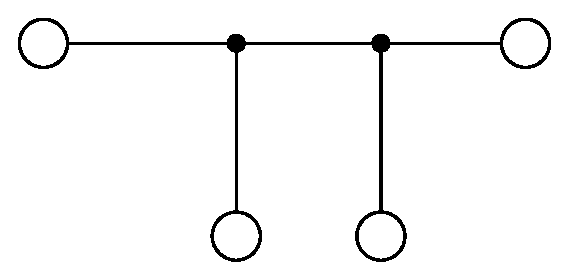
\includegraphics[]{pics/1b.eps}
                \caption{Вариант дерева для четырех терминалов и двух перекрестков}
            \end{figure}
        \end{enumerate}
        
        Попытка добавить большее количество перекрестков приведет просто к тому, что на самом деле это будет не перекресток, а вершина какого-то пути, но и в целом, я надеюсь, что из ``итеративной'' процедуру присоединения новых терминалов видно, что мы как бы выпускаем лучик из терминала. 
        Этот лучик может врезаться в терминал, тогда не очень интересно; может врезаться в перекресток, а может врезаться, например, в путь, тогда образуется новый перекресток.
        
        Стоит отметить, что случай, когда у нас новый перекресток образуется не на пути, а где-то в вакууме через аналогию с лучиком не очень хорошо понимается, только если Вы не знаете случайно КЭД и что лучик может умереть, ни с чем не столкнувшись :)

        К слову еще одно замечание, которое не прозрачно из предыдущего: в случае вырождения (то есть когда перекрестки либо совпадают друг с другом, либо с терминалом(ами)) мы перебираем еще всевозможные соединения (опять же в смысле соединения путями) этих вершин, то есть в каком-то смысле перебираем такие деревья.
    \end{upd}
\end{solution}